\documentclass[11pt]{article}
\usepackage[margin=1in]{geometry}
\usepackage{textcomp}
\usepackage{gensymb}
\usepackage{graphicx}
\usepackage{caption}
\usepackage{epstopdf}
\usepackage{textgreek}
\usepackage{titlesec}
\usepackage{float}
\usepackage{cite}
%\usepackage{natbib}
\usepackage[articletitle=true,doi=true]{achemso}

\titlespacing*{\section} {0pt}{0mm}{0mm}
\titlespacing*{\subsection} {0pt}{0mm}{0mm}

\let\bf\textbf

\begin{document}
\linespread{1.25}
\raggedright
\setlength{\parskip}{2pt}
\setlength{\belowcaptionskip}{-8pt}
%\captionsetup{belowskip=0pt}
\def\citenumfont{\textnormal}
\renewcommand{\bibsection}{}

\subsection*{INTRODUCTION}
The Diels-Alder reaction is a prominent pericyclic reaction in organic chemistry that is able to reliably form cyclohexene rings with predictable regio- and stereochemistry under relatively simple conditions.\cite{Brocksom2001} The reaction occurs between a conjugated diene, and dienophile and proceeds via a concerted [4+2] cycloaddition, the simplicity of which allows for a considerable amount of synthetically useful reactions.\cite{Nicolaou2002} In addition to the classic Diels-Alder reaction, there are a number of related variants including the intramolecular Diels-Alder reaction, capable of forming bridged and fused polycyclic adducts, the hetero-Diels-Alder reaction which can form a variety of heterocycles, and the hexadehydro Diels-Alder reaction, an analogous alkyne reaction which able to form substituted benzene compounds.\cite{Heravi2015,Hoye2012} There is even evidence of enzymes capable of mediating Diels-Alder reactions in biosynthetic pathways.\cite{Stocking2003} As such it has applications in a wide range of disciplines including the industrial production of pharmaceuticals and agrochemicals, the total synthesis of natural products, and polymer chemistry among others.\cite{Funel2013,Nicolaou2002,Briou2021}  Of the many diene/dienophile pairs that have been investigated, the reaction between furan and maleimide has been the most studied due to its application in polymer chemistry.\cite{Briou2021} This popularity is in large part due to the convenient temperature range of Diels-Alder/retro-Diels-Alder equilibrium of the reaction, and low possibility of side reactions or thermal degradation.\cite{Gandini2013} These properties have been exploited to produce cross-linked polymeric material capable of re-mending under mild conditions.\cite{Chen2002} A sizeable amount of research has also been put into the application of furan/maleimide polymers with epoxy functionalities in order to develop thermally removable epoxy adhesives.\cite{Mcelhanon2002} Another opposite approach involves the transformation of the Diels-Alder adduct by an aromatization reaction to produce highly thermostable polymers.\cite{Gandini2013} This process is irreversible and produces polymers that are stable at temperatures well above those which favor retro-Diels-Alder reactions in the original adducts.\cite{Tesoro1986} The furan/maleimide combination is also advantageous in terms of green chemistry as there is some interests in the use of furan compounds derived from renewable sources.\cite{Gandini2008} The maleimide component can be obtained in a relatively simple two-step synthesis involving the reaction of maleic anhydride and amines followed by dehydration.\cite{Briou2021} In this paper, we present a green synthesis of \textit{N}-phenylmaleimide precursors by utilizing a solvent free room temperature reaction in the formation of the maleimide, and demonstrate its use as a dienophile in furan/maleimide Diels-Alder reactions. This contributes to the already sizeable body of knowledge on furan/maleimide Diels-Alder reactions, and presents a greener alternative to more traditional synthetic methods. 

\subsection*{METHODS AND RESULTS}
\bf{Chemicals.} 4-chloroaniline, maleic anhydride, acetic anhydride, sodium acetate, 2,5-dimethylfuran were used as recieved without further purification.

\bf{Instrumentation.} Nuclear magnetic resonance (NMR) spectra were recorded on a Bruker Ultrashield™ (CDCl$_3$, 400 MHz) calibrated using deuterated solvent (CDCl$_3$: $^1$H NMR: 7.26 ppm). IR spectra were recorded on a Nicolet Summit™ FTIR spectrometer. UV-Vis spectra were recorded on a Vernier Fluorescence/UV-Vis spectrophotometer.

\begin{figure}[H]
    \centering
    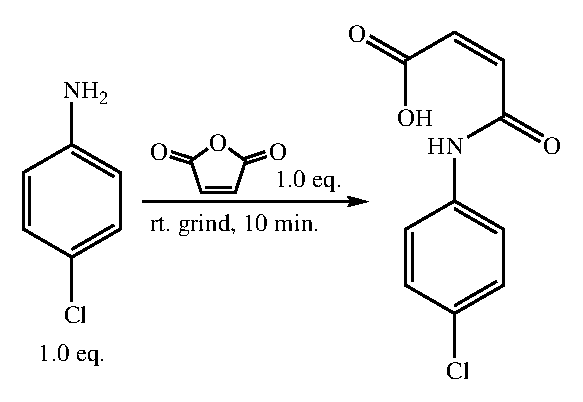
\includegraphics[scale=0.8]{schemes/scheme1.eps}
    \caption*{Scheme 1: Solvent-free Synthesis of \textit{N}-(4-chloro)maleanilic acid}
\end{figure}

\bf{Procedure.} Maleic anhydride (0.98 g, 10 mmol) was melted in a mortar on a hot plate. Once melted the mortar was removed from heat and 4-chloroaniline (1.28 g, 10 mmol) was added. The resulting mixture was then ground for 10 minutes transferred to a small beaker with 10 mL EtOAc and stirred for one minute. The product was then filtered by vacuum, washed on the filter with EtOAc, and air dried.

\bf{\textit{N}-(4-chloro)maleanilic acid:} bright yellow powder. Hexanes:EtOAc 1:1 R\textsubscript{f} = 0.43. \bf{\textsuperscript{1}H-NMR} (400 MHz) \textdelta\; 6.299 - 6.329 (d, 1H), 6.456 - 6.486 (d, 1H), 7.381 - 7.403 (d, 2H), 7.644 - 7.666 (d, 2H), 10.462 (s, 1H). \bf{IR} (Neat): 3080, 1893, 1702, 1630, 1487, 1398, 1094 cm$^{-1}$. \bf{UV-Vis:} \textlambda\textsubscript{max} = 295.5 nm. \bf{Yield:} (1.100 g, 48.8\%)

\begin{figure}[H]
    \centering
    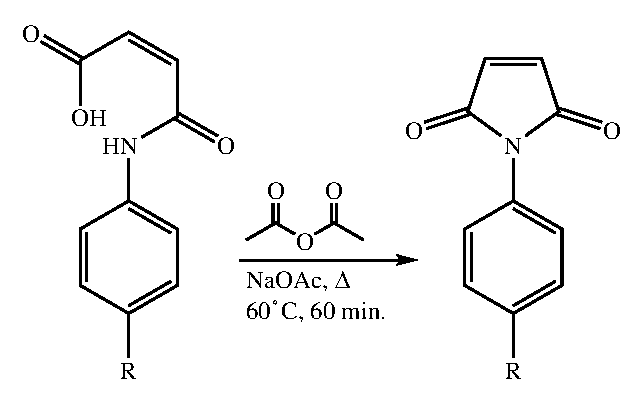
\includegraphics[scale=0.8]{schemes/scheme2.eps}
    \caption*{Scheme 2: Synthesis of \textit{N}-(4-chlorophenyl)maleimide}
\end{figure}

\bf{Procedure.} To a 50 mL round bottom flask was added \textit{N}-(4-chloro)maleanilic acid (1.100 g, 4.88 mmol), sodium acetate (0.15 g, 1.83 mmol), and acetic anhydride (3 mL, 31.7 mmol). The solution was placed in a hot water bath and held at 60\degree C for 60 minutes. When the reaction was complete, the reaction mixture was transferred to a beaker containing 50 mL ice-cold DI H$_2$O and stirred for \textasciitilde 5 minutes. The solid precipitate was then filtered by vacuum, recrystallized from EtOH, and air dried.

\bf{\textit{N}-(4-chlorophenyl)maleimide:} yellow powder. Hexanes:EtOAc 1:1 R\textsubscript{f} = 0.32. \bf{\textsuperscript{1}H-NMR} (400 MHz) \textdelta\; 6.865 (s, 2H), 7.300 - 7.336 (dt, 2H), 7.424 - 7.460 (dt, 2H). \bf{IR} (Neat): 1710, 1496, 1385, 1146, 1095 cm$^{-1}$ \bf{UV-Vis:} \textlambda\textsubscript{max} = 309.4 nm. \bf{Yield:} (0.578 g, 57.1\%)

\begin{figure}[H]
    \centering
    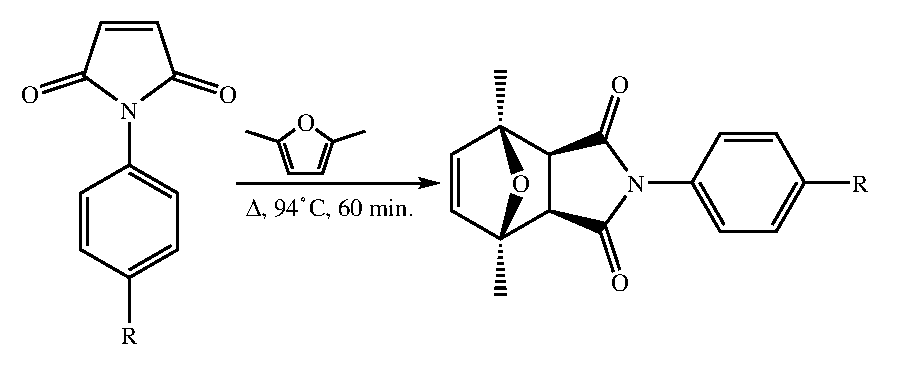
\includegraphics[scale=0.8]{schemes/scheme3.eps}
    \caption*{Scheme 3: Diels-Alder reaction of \textit{N}-(4-chlorophenyl)maleimide and 2,5-dimethylfuran}
\end{figure}

\bf{Procedure.} To a 3 mL conical vial was added \textit{N}-(4-chlorophenyl)maleimide (0.100 g, 0.44 mmol) and 2,5-dimethylfuran (1.0 mL, 9.3 mmol). The resulting mixture was heated to 94\degree C and held at reflux for 60 minutes. When the reaction was complete the solution was cooled to room temperature, placed in an ice bath to precipitate, then filtered by vacuum and recrystallized from EtOH. 

\bf{2-(4-chlorophenyl)-4,7-dimethyl-3a,4,7,7a-tetrahydro-1H-4,7-epoxyisoindole-1,3(2H)-dione:} yellow crystals. \bf{\textsuperscript{1}H-NMR} (400 MHz) \textdelta\; 1.764 (s, 6H), 6.369 (s, 2H), 7.237 - 7.242 (d, 2H), 7.424 - 7.430 (d, 2H), 7.446 - 7.453 (d, 2H). \bf{IR} (Neat): 2981, 1702, 1494, 1386, 1200, 1090 cm$^{-1}$ \bf{UV-Vis:} \textlambda\textsubscript{max} = 252.9 nm. \bf{Yield:} (0.230 g, 172.1\%)

\subsection*{DISCUSSION}
\bf{\textit{N}-(4-chloro)maleanilic acid.} The final yield was 1.100 g corresponding to a percent yield of 48.8\%. The experimental NMR spectrum showed 2 doublet peaks with an integration of 1 corresponding to the hydrogens of maleic anhydride and 2 doublet peaks with an integration of 2 corresponding to the two sets of identical aromatic hydrogens indicating \textit{para} substitution. Another singlet peak was observed at 10.462 ppm likely corresponding to the amide functional group. No singlet peak was observed for the carboxylic acid O-H proton, potentially due to water remaining in the sample.

\bf{\textit{N}-(4-chlorophenyl)maleimide.} The final yield was 0.578 g, corresponding to a percent yield of 57.1\%. The experimental NMR spectrum showed two doublet of triplet peaks with integration of 2 corresponding to the two sets of aromatic hydrogens, and a singlet peak with an integration of 1, corresponding to the two hydrogens of the maleimide functional group. 

\bf{2-(4-chlorophenyl)-4,7-dimethyl-3a,4,7,7a-tetrahydro-1H-4,7-epoxyisoindole-1,3(2H)-dione.} The final yield was 0.230 g corresponding to a percent yield of 172.1\% due to incomplete drying. The experimental NMR spectrum showed a singlet peak with an integration of 6 corresponding to the methyl groups from 2,5-dimethylfuran, as well as two doublet peaks with an integration of 1 corresponding to the two pairs of aromatic hydrogens. The experimental IR spectrum showed a strong C=O stretching peak at 1702 cm$^{-1}$ which was considerably stronger than the equivalent peak in the IR spectrum of \textit{N}-(4-chlorophenyl)maleimide. 

\newpage
\subsection*{REFERENCES}
\vspace{2mm}
\bibliography{references}

\newpage
\subsection*{APPENDIX A: SPECTRA}

%%% NMR SPECTRA %%%
\begin{figure}[H]
    \centering
    \includegraphics[scale=0.105]{spectra/nmr9.1.png}
    \caption{\textit{N}-(4-chloro)maleanilic acid NMR Spectrum}
\end{figure}
\begin{figure}[H]
    \centering
    \includegraphics[scale=0.105]{spectra/nmr9.2.png}
    \caption{\textit{N}-(4-chlorophenyl)maleimide NMR Spectrum}
\end{figure}
\begin{figure}[H]
    \centering
    \includegraphics[scale=0.105]{spectra/nmr9.3.png}
    \caption{2-(4-chlorophenyl)-4,7-dimethyl-3a,4,7,7a-tetrahydro-1H-4,7-epoxyisoindole-1,3\\(2H)-dione NMR}
\end{figure}

\newpage

%%% IR SPECTRA %%%
\begin{figure}[H]
    \centering
    \includegraphics[scale=0.33]{spectra/ir9.1.png}
    \caption{\textit{N}-(4-chloro)maleanilic acid IR Spectrum}
\end{figure}
\begin{figure}[H]
    \centering
    \includegraphics[scale=0.33]{spectra/ir9.2.png}
    \caption{\textit{N}-(4-chlorophenyl)maleimide IR Spectrum}
\end{figure}
\begin{figure}[H]
    \centering
    \includegraphics[scale=0.33]{spectra/ir9.3.png}
    \caption{IR Spectrum}
\end{figure}
\begin{figure}[H]
    \centering
    \includegraphics[scale=0.33]{spectra/ir10.1.png}
    \caption{\textit{N}-(4-methyl)maleanilic acid IR Spectrum}
\end{figure}
\begin{figure}[H]
    \centering
    \includegraphics[scale=0.33]{spectra/ir10.2.png}
    \caption{\textit{N}-(4-methylphenyl)maleimide IR Spectrum}
\end{figure}
\begin{figure}[H]
    \centering
    \includegraphics[scale=0.33]{spectra/ir10.3.png}
    \caption{ IR Spectrum}
\end{figure}

%%% UV-VIS SPECTRA %%%
\begin{figure}[H]
    \centering
    \includegraphics[scale=0.33]{spectra/uvvis9.1.png}
    \caption{\textit{N}-(4-chloro)maleanilic acid UV-Vis Spectrum}
\end{figure}
\begin{figure}[H]
    \centering
    \includegraphics[scale=0.33]{spectra/uvvis9.2.png}
    \caption{\textit{N}-(4-chlorophenyl)maleimide UV-Vis Spectrum}
\end{figure}
\begin{figure}[H]
    \centering
    \includegraphics[scale=0.33]{spectra/uvvis9.3.png}
    \caption{ UV-Vis Spectrum}
\end{figure}
\begin{figure}[H]
    \centering
    \includegraphics[scale=0.33]{spectra/uvvis10.1.png}
    \caption{\textit{N}-(4-methyl)maleanilic acid UV-Vis Spectrum}
\end{figure}
\begin{figure}[H]
    \centering
    \includegraphics[scale=0.33]{spectra/uvvis10.2.png}
    \caption{\textit{N}-(4-methylphenyl)maleimide UV-Vis Spectrum}
\end{figure}
\begin{figure}[H]
    \centering
    \includegraphics[scale=0.33]{spectra/uvvis10.3.png}
    \caption{ UV-Vis Spectrum}
\end{figure}

\end{document}